\documentclass{aes53i}
\hyphenation{Post-Script}


\usepackage{graphicx}
\usepackage{amssymb}

\usepackage{xcolor}
%\usepackage{hyperref} % Apparemment pas compatible avec le style AES !!
\usepackage{url}
\usepackage[utf8]{inputenc}
\usepackage[T1]{fontenc}

\usepackage{enumitem}
\setlist{nosep}

\setlength{\parskip}{0pt}

%----------
%  Header
%----------


% first the title is needed
\title{Telemeta : open web audio platform for sound archives in the use case of ethnomusicology}

% a short form should be given in case it is too long for the running head
\shorttitle{Telemeta : open web audio platform for sound archives}

\author{
  Thomas Fillon\aff{1,2},
  Guillaume Pellerin\aff{1},
  Paul Brossier\aff{1},
  and Jos{\'e}phine Simonnot\aff{3} 
\thanks{This work was partially done inside the DIADEMS project funded by the national french agency ANR (CONTINT)}
}


\affiliation[1]{PARISSON, 16 rue Jacques Louvel-Tessier 75010 Paris, France}
\affiliation[2]{LAM, Institut Jean Le Rond d'Alembert, UPMC Univ. Paris 06, UMR CNRS 7190, 11 rue de Lourmel, 75015 Paris, France}
\affiliation[3]{
CREM, LESC, UMR CNRS 7186, MAE, Université Paris Ouest Nanterre La Défense,
21 Allée de l'Université - 92023 Nanterre}

\correspondence{Thomas Fillon and Guillaume Pellerin}{thomas.fillon@parisson.com, guillaume.pellerin@parisson.com}

\lastnames{Fillon, Pellerin, Brossier, Simonnot}

%\url{josephine.simonnot@mae.u-paris10.fr}}



\begin{abstract}
\emph{Telemeta} is a fully-operational open-source web audio platform dedicated to digital sound archives secure storing, indexing and publishing. It focuses on the enhanced and collaborative user-experience in accessing audio items and their associated metadata and on the possibility for the expert users to further enrich those metadata.

Telemeta architecture relies on \emph{TimeSide}, an open audio processing framework written in Python which provides decoding,  encoding and streaming methods for various formats together with a smart embeddable HTML audio player. TimeSide also includes a set of audio analysis plugins and additionally wraps several audio features extraction libraries to provide automatic annotation, segmentation and musicological analysis.

The demonstration presents the features of this platform in the context of ethnomusicological research.
\end{abstract}

\begin{document}
\maketitle

\section{Introduction}

 % In social sciences like anthropology and linguistics, researchers have to work on multiple types of multimedia documents such as photos, videos, sound recordings or databases. The need to easily access, visualize and annotate such materials can be problematic given their diverse formats, sources and given their chronological nature.
  %With this in mind, some laboratories\footnote{The Research Center on Ethnomusicology (CREM), the Musical Acoustics Laboratory (LAM, UMR 7190) and the sound archives of the Mediterranean House of Human Sciences (MMHS)} involved in ethnomusicological research have been working together on that issue.

  In the context of ethnomusicological research, the Research Center on Ethnomusicology 
(CREM) and Parisson, a company specialized in the management of audio databases, have been developing an innovative, collaborative and interdisciplinary open-source web-based multimedia platform since 2007. This platform, \emph{Telemeta} is designed to fit the professional requirements from both sound archivists and researchers in ethnomusicology. The first prototype of this platform has been online\footnote{Archives sonores du CNRS, Musée de l'Homme, http://archives.crem-cnrs.fr} since 2008.

 \section{Telemeta}\label{sec:Telemeta}
 \subsection{Web audio content management features and architecture}
 Telemeta\footnote{http://telemeta.org} is a free and open source\footnote{Telemeta code is available under the CeCILL Free Software License Agreement \texttt{http://cecill.info/licences/Licence\_CeCILL\_V2-en.html}} web audio platform which introduces efficient and secure methods for back-uping, indexing, transcoding, analysing and publishing any digitalized audio file with its metadata. 

% An overview of the Telemeta's web interface is illustrated in Figure~\ref{fig:Telemeta}
% \begin{figure}
%   \centering
%   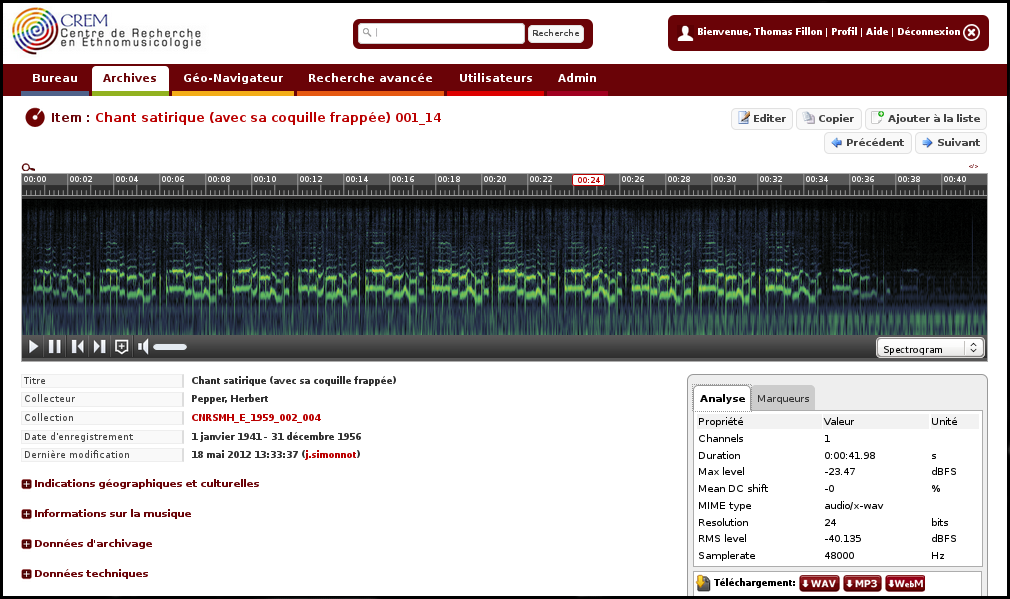
\includegraphics[width=0.95\linewidth]{img/telemeta.png}
%   \caption[1]{Screenshot excerpt of the \emph{Telemeta} web interface}
%    \label{fig:Telemeta}
% \end{figure}

Telemeta is ideal for professionals who wants to easily organize, backup, archive and publish documented sound collections of audio files, CDs, digitalized vinyls and magnetic tapes over a strong database, in accordance with open web standards. 
\emph{Telemeta} architecture is flexible and can easily be adapted to particular database organization of a given sound archives. 

The main features of \emph{Telemeta} are:
\begin{itemize}
\item \emph{Pure HTML} web user interface including high level \emph{search engine}
\item Smart \emph{workflow management} with contextual user lists, profiles and rights
  % \item RSS and JSON feed generators
  % \item XML serialized backup
\item Strong Structured Query Language (SQL) or Oracle backend
\item Model-View-Controller (MVC) architecture 
\end{itemize}
Beside database management, the audio support is mainly provided through an external component, TimeSide, which is described in Section~\ref{sec:Timeside}.

\subsection{Metadata}\label{sec:metadata}
In addition to the audio data, an efficient and dynamic management of the associated metadata is also required. %Consulting metadata provide both an exhaustive access to valuable information about the source of the data and to the related work of peer researchers. 
Dynamically handling metadata in a collaborative manner optimises the continuous process of knowledge gathering and enrichment of the materials in the database.  
%One of the major challenge is thus the standardization of audio and metadata formats with the aim of long-term preservation and usage of the different materials.
The compatibility with other systems is facilitated by the integration of the metadata standards protocols \emph{Dublin Core} and \emph{OAI-PMH} (Open Archives Initiative Protocol for Metadata Harvesting) \cite{DublinCore,OAI-PMH}.

Metadata provide two different kinds of information about the audio item: contextual information and annotations.
\vspace{-0.4cm}

\paragraph{Contextual Information}
In ethnomusicology, contextual information could be geographic, cultural and musical. It could also store archive related information and include related materials in any multimedia format.
\vspace{-0.4cm}
\paragraph{Annotations and segmentation}
Metadata also consist in temporal information such as a list of \emph{time-coded markers} associated with annotations and a list of of \emph{time-segments} associated with labels. The ontology for those labels is relevant for ethnomusicology (e.g. speech versus singing voice segment, chorus, ...).
It should be noted that annotations and segmentation can be done either by a human expert or by some automatic signal processing analysis (see Section~\ref{sec:Timeside}).

\section{TimeSide}\label{sec:Timeside}
One specificity of the Telemeta architecture is to rely on an external component, \emph{TimeSide}\footnote{\url{https://github.com/yomguy/TimeSide}}, that offers audio player web integration together with audio signal processing analysis capabilities. 

% Figure~\ref{fig:TimeSide_Archi} illustrates the overall architecture of \emph{TimeSide}.

% \begin{figure}[htbp]
%   \centering
%   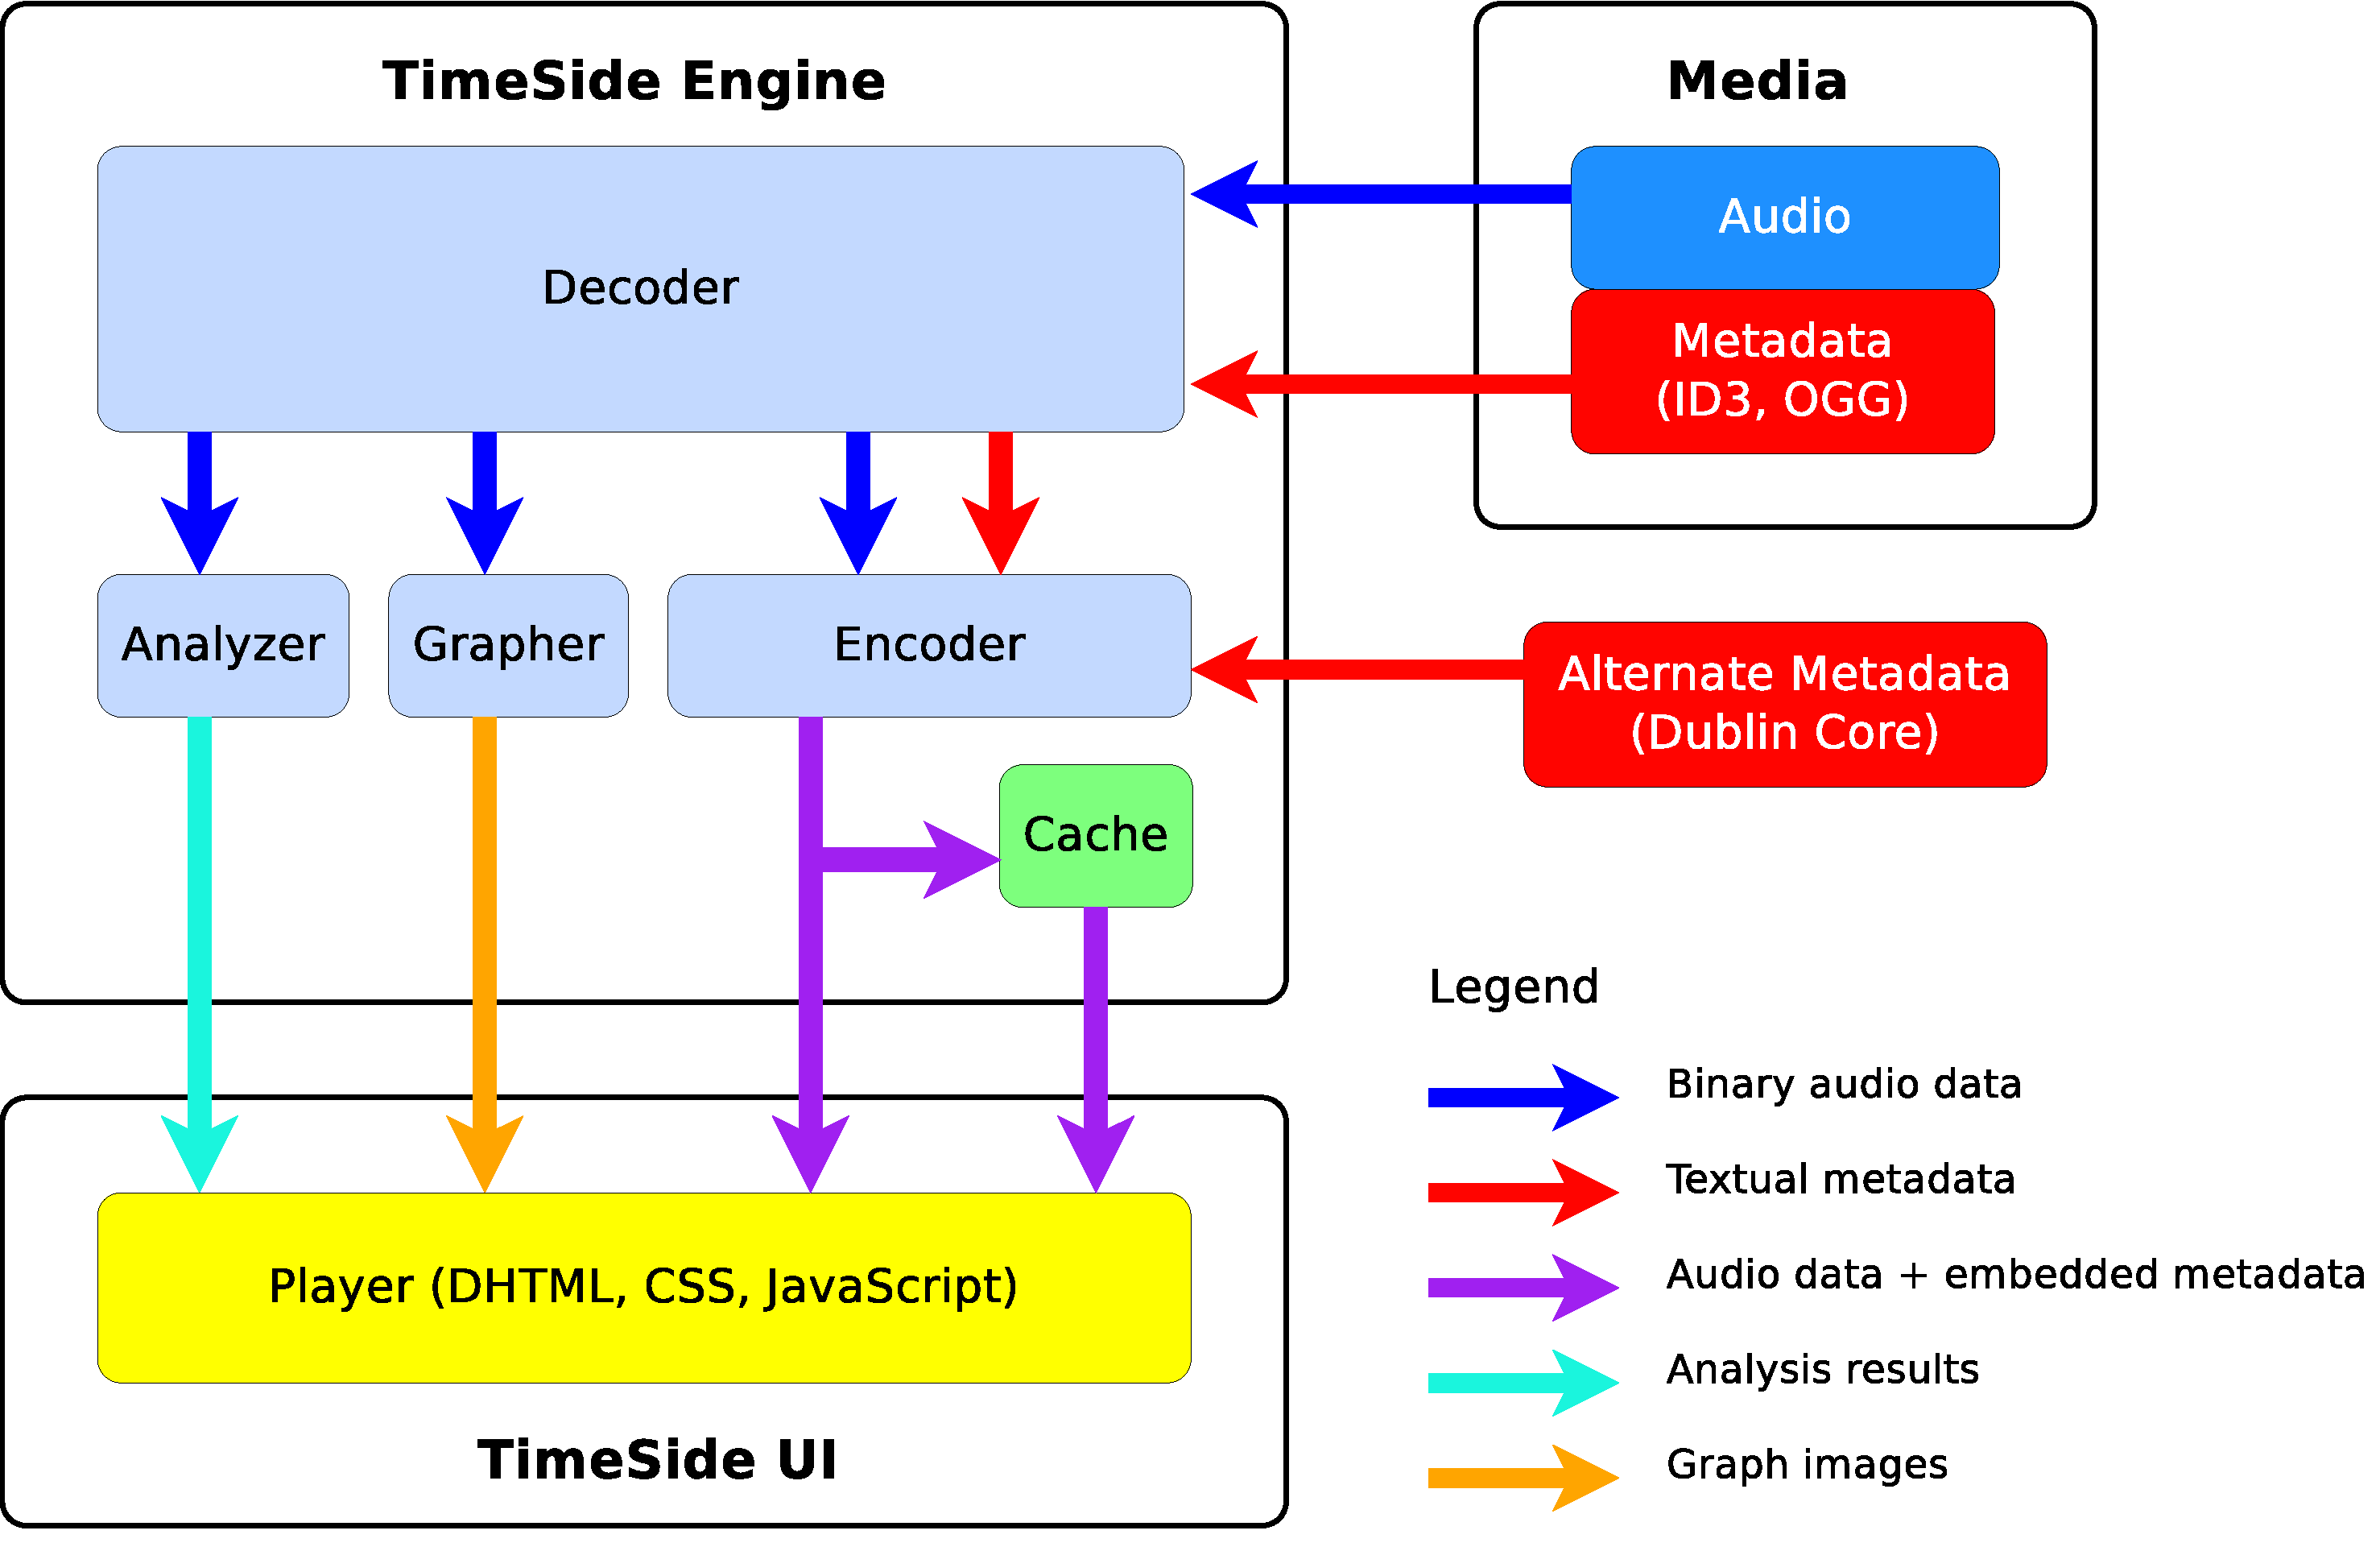
\includegraphics[width=0.95\linewidth]{img/timeside_schema.pdf}
%   \caption{TimeSide architecture (see \texttt{https://code.google.com/p/timeside/})}\label{fig:TimeSide_Archi}
% \end{figure}


\subsection{Audio management}
TimeSide provides the following main features:
\begin{itemize}
\item \emph{Secure archiving, editing and publishing of audio files} over
  internet.
\item Smart \emph{audio player} with enhanced visualisation (waveform, spectrogram)
\item \emph{Multi-format support}: reads all available audio and video formats  through Gstreamer, transcoding with smart streaming and caching methods% (FLAC, OGG, MP3, WAV and WebM)
  % \item \emph{Playlist management} for all users with CSV data export
\item "On the fly" \emph{audio analyzing, transcoding and metadata
    embedding} based on an easy plugin architecture
\end{itemize}

\subsection{Audio features extraction}
TimeSide incorporates some state-of-the-art audio feature extraction libraries such as Aubio\footnote{\url{http://aubio.org/}}, Yaafe\footnote{\url{http://yaafe.sourceforge.net}} and Vamp plugins\footnote{ \url{http://www.vamp-plugins.org}} \cite{brossierPhD,yaafe_ISMIR2010,vamp-plugins}.
Given the extracted features, every sound item in a given collection can be automatically analyze. The results of this analysis can be stored in a scientific file format (\emph{Numpy}, \emph{HDF5}) and serialized to the web browser through commons markup languages (\emph{xml}, \emph{json}, \emph{yaml}).
Further works lead by the DIADEMS project will incorporate advance Music Information Retrieval methods in order to provide automatic annotation, segmentation and similarity analysis.

\section{Conclusion - Purpose of the demonstration}\vspace{-0.1cm}
The demonstration presents the features offered by \emph{Telemeta} as detailed in Section~\ref{sec:Telemeta} in the context of ethnomusicological sound archiving.%\cite{telemetaCREM} 
It focuses on the enhanced and collaborative user-experience when accessing audio items and their associated metadata, and on the possibility for the expert user to further enrich those metadata.
Another goal of this demonstration is to present the integrated audio analysis tools described in Section~\ref{sec:Timeside}.
\vspace{-0.2cm}
\section*{Acknowledgments} 
{\small The authors would like to thank all the people that have been involved in \emph{Telemeta} specification and development or have provide useful input and feedback. 
The project has been partially funded by the French National Centre for Scientific Research (CNRS), the French Ministry of Culture and Communication, the TGE Adonis Consortium, and the Centre of Research in Ethnomusicology (CREM).}


\bibliographystyle{plain}
\bibliography{aes53_Telemeta}


\end{document}
